\documentclass[conference]{IEEEtran}

\usepackage{fontspec}
\setmainfont{texgyretermes-regular.otf}[
  BoldFont=texgyretermes-bold.otf,
  ItalicFont=texgyretermes-italic.otf,
  BoldItalicFont=texgyretermes-bolditalic.otf
]
\usepackage{booktabs}
\usepackage{balance}
\usepackage{array}
\usepackage{microtype}
\usepackage{tikz}
\usetikzlibrary{arrows.meta,positioning,calc}
\usepackage{url}
\usepackage[hidelinks]{hyperref}

\hypersetup{
  pdftitle={Confirmation-Gated HIL Fault-Injection Trials for Auditable Payload-Link Supervision},
  pdfauthor={},
  pdfsubject={},
  pdfkeywords={hardware-in-the-loop, fault injection, embedded systems, payload link, reproducibility}
}

\title{Confirmation-Gated HIL Fault-Injection Trials for Auditable Payload-Link Supervision}
\author{}

\begin{document}
\maketitle

\begin{abstract}
An injection request does not show that the requested condition became active at the injected endpoint. This distinction matters when controller detection and recovery are scored from separate observations. We present a confirmation-gated hardware-in-the-loop (HIL) trial protocol for a supervised payload link. Payload-side confirmation of the injected condition gates detection scoring, and payload-side confirmation of NORMAL restoration gates recovery scoring. Requested, activated, detected, restored, and recovered events remain separate in byte-preserving controller and payload traces. In a setup-bounded demonstration, one G431/G474 pair completed 90 sequential trials, 30 each for silence, bad CRC, and delay. All 90 trials had confirmed activation and restoration; the predefined detector and recovery markers appeared in 30/30 valid trials per mode. Host-observed median command-to-marker intervals ranged from 359.5 to 406.0~ms for detection and from 296.5 to 359.0~ms for recovery. Separate evidence comprises a 605-s nominal observation, two BAD\_CRC mechanism observations, and two 12-row F411 pair campaigns reported with separate denominators. The results demonstrate the protocol on the evaluated setups. They are not reliability, device-population, MCU-equivalence, or controller-internal timing estimates.
\end{abstract}

\begin{IEEEkeywords}
hardware-in-the-loop, fault injection, embedded systems, payload link, reproducibility
\end{IEEEkeywords}

\section{Introduction}

Embedded controllers often supervise whether a peripheral responds, whether a received frame is valid, and whether an unavailable peer returns to service. HIL fault injection can exercise these paths, but its evidence is ambiguous if a sent injector command is treated as proof of endpoint activation. The same problem recurs at recovery: requesting restoration does not show that the endpoint returned to its normal behavior. Controller markers should be scored only after those endpoint facts are separately observed.

Fault-injection methodology distinguishes faults, functional activation, readouts, and measures~\cite{arlat1990}. Automotive HIL work provides programmatic signal faults, logging, and automated evaluation~\cite{abboush2022,abboush2024}. Nanosatellite work injects communication-bus faults and reuses interoperability tests across MIL and HIL settings~\cite{batista2019,conceicao2025}. Among the closest published studies reviewed, we did not find a payload-link trial protocol that gates detector scoring on separate payload-side confirmation of the injected condition, gates recovery scoring on separate payload-side confirmation of NORMAL restoration, and retains the five resulting event classes as separately auditable records.

We therefore propose a confirmation-gated experimental protocol. A command is a request, not activation evidence. Separate payload-side observation establishes activation or restoration; only then can a controller-side detector or recovery marker be scored. Both endpoint streams retain host timestamps, exact received bytes, and readable renderings. Hash-verified frozen summaries provide the inputs to manuscript tables.

The paper makes three bounded contributions, in priority order:

\begin{itemize}
  \item a confirmation-gated trial protocol that separates requested, activated, detected, restored, and recovered events and makes missing confirmation invalidate rather than fail a trial;
  \item an auditable evidence workflow that retains byte-preserving endpoint traces and verifies frozen summaries and table inputs with SHA-256; and
  \item a setup-bounded descriptive evaluation using one G431/G474 pair for 90 primary trials, a separate 605-s nominal observation, two BAD\_CRC mechanism observations, and two separate 12-row F411 pair campaigns.
\end{itemize}

The evaluated firmware and boards are context, not an architecture contribution or a new HIL framework, injector, simulator, or fault model. The study does not claim comparative advantage, reliability, population generality, flight qualification, mission assurance, MCU-family equivalence, or complete-system validation.

\begin{figure*}[!t]
\centering
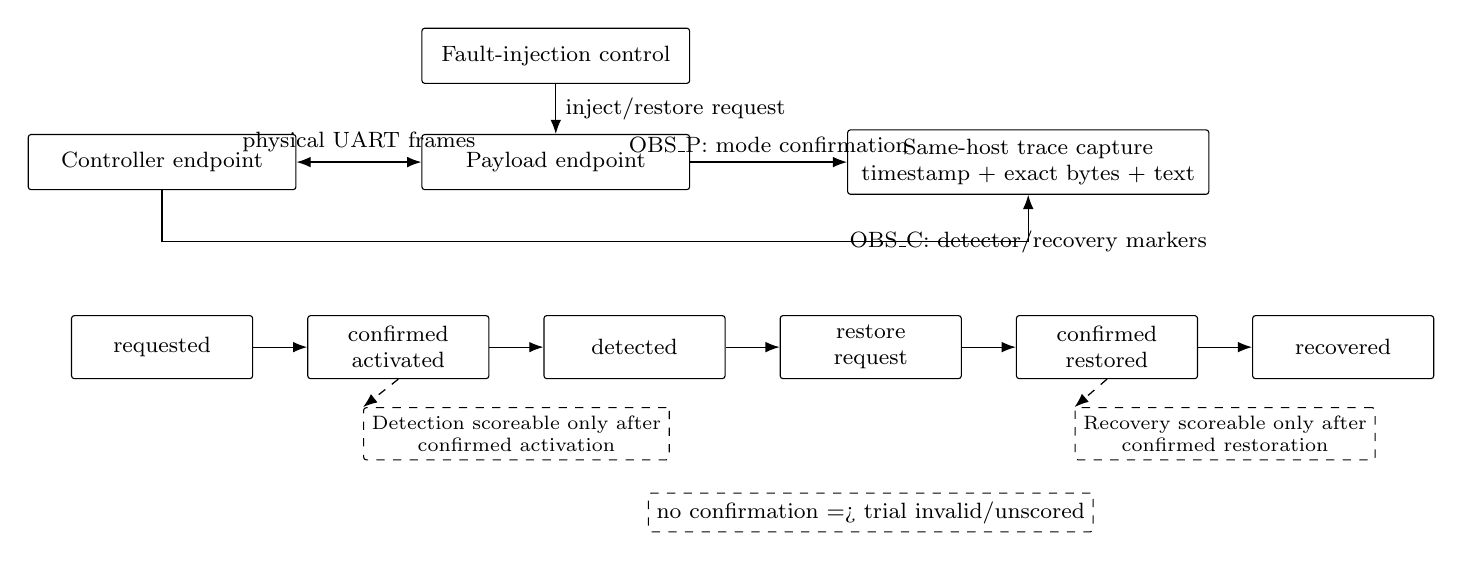
\begin{tikzpicture}[
  font=\footnotesize,
  box/.style={draw,rounded corners=1pt,align=center,minimum height=7mm,inner xsep=5pt},
  event/.style={box,minimum width=23mm,minimum height=8mm},
  flow/.style={-{Latex[length=1.8mm]},line width=0.45pt},
  link/.style={{Latex[length=1.8mm]}-{Latex[length=1.8mm]},line width=0.45pt},
  gate/.style={draw,dashed,rounded corners=1pt,align=center,font=\scriptsize,inner sep=3pt}
]
  \node[box,minimum width=34mm] (ctrl) at (0,0) {Controller endpoint};
  \node[box,minimum width=34mm] (payload) at (5.0,0) {Payload endpoint};
  \node[box,minimum width=34mm] (inject) at (5.0,1.35) {Fault-injection control};
  \node[box,minimum width=43mm] (trace) at (11.0,0) {Same-host trace capture\\timestamp + exact bytes + text};
  \draw[link] (ctrl.east) -- node[above]{physical UART frames} (payload.west);
  \draw[flow] (inject.south) -- node[right]{inject/restore request} (payload.north);
  \draw[flow] (payload.east) -- node[above]{OBS\_P: mode confirmation} (trace.west);
  \draw[flow] (ctrl.south) -- ++(0,-0.65) -| node[pos=0.72,below]{OBS\_C: detector/recovery markers} (trace.south);

  \node[event] (requested) at (0,-2.35) {requested};
  \node[event] (activated) at (3.0,-2.35) {confirmed\\activated};
  \node[event] (detected) at (6.0,-2.35) {detected};
  \node[event] (restoreq) at (9.0,-2.35) {restore\\request};
  \node[event] (restored) at (12.0,-2.35) {confirmed\\restored};
  \node[event] (recovered) at (15.0,-2.35) {recovered};
  \draw[flow] (requested) -- (activated);
  \draw[flow] (activated) -- (detected);
  \draw[flow] (detected) -- (restoreq);
  \draw[flow] (restoreq) -- (restored);
  \draw[flow] (restored) -- (recovered);

  \node[gate] (dg) at (4.5,-3.45) {Detection scoreable only after\\confirmed activation};
  \node[gate] (rg) at (13.5,-3.45) {Recovery scoreable only after\\confirmed restoration};
  \draw[flow,dashed] (activated.south) -- (dg.north west);
  \draw[flow,dashed] (restored.south) -- (rg.north west);
  \node[gate,font=\footnotesize] at (9.0,-4.45) {no confirmation => trial invalid/unscored};
\end{tikzpicture}
\caption{Confirmation-gated topology and event sequence. OBS\_C and OBS\_P are separate same-host channels. Arrows define scoring stages, not controller states or strict host-receipt-time order.}
\label{fig:protocol}
\end{figure*}

\section{Related Work}

Arlat \emph{et al.} define a fault-injection experiment through a fault, an activation trajectory, a readout, and derived measures (FARM)~\cite{arlat1990}. Their activation set functionally exercises the system; separate endpoint confirmation that a requested condition became active is not reported in the cited publication. The distinction here is narrower: activation is an observed payload state that gates whether the controller readout may enter the score.

Abboush \emph{et al.} configure fault type, location, time, and duration in real-time automotive HIL experiments and record system signals for evaluation~\cite{abboush2022}. Their later framework automates campaigns across virtual driving scenarios and reports fault deactivation followed by return toward a safe state~\cite{abboush2024}. Separate injected-endpoint confirmation before detection scoring and separate restoration confirmation before recovery scoring are not reported in the cited publications.

At the communication boundary, Batista \emph{et al.} describe a COTS failure-emulator mechanism that intercepts and changes nanosatellite I$^2$C traffic for MIL/HIL robustness tests~\cite{batista2019}. Concei\c{c}\~ao and Mattiello-Francisco organize interoperability testing into six MIL, SIL, and HIL modules, reuse model-derived tests, and employ that mechanism for bus faults~\cite{conceicao2025}. These publications report injection, subsystem observations, and test traceability. The cited publications do not report confirmation-gated scoring with all requested, activated, detected, restored, and recovered events kept distinct, nor byte-preserving endpoint traces feeding hash-verified frozen summaries. ``Not reported'' is limited to these publications and is not a claim about all prior work.

\section{System Context and Protocol}

\subsection{Evaluated Link}

The primary setup connects a NUCLEO-G431RB controller to a NUCLEO-G474RE payload simulator by a 115200~8N1 UART with common ground. The controller polls the payload and exposes timeout, rejection, OFFLINE, and recovery markers. The commandable payload returns NORMAL responses, withholds responses in SILENT mode, corrupts response CRCs in BAD\_CRC mode, and delays responses by 250~ms in DELAYED mode. The inspected controller deadline is 100~ms.

As Fig.~\ref{fig:protocol} shows, the host sends fault-control commands and separately captures controller (OBS\_C) and payload (OBS\_P) serial streams. These are separate observation channels collected on the same host; no stronger host or statistical independence is implied. The topology is the minimum context needed to define the protocol.

\subsection{Validity and Scoring}

For trial $i$, let $A_i$ denote payload confirmation of the requested injected condition and $S_i$ payload confirmation of restored NORMAL. The trial is valid for complete scoring only if $V_i=A_i\land S_i$ and no harness invalid reason is present. Detection is evaluated only after $A_i$; recovery is evaluated only after $S_i$. Thus, missing activation or restoration confirmation makes the affected trial invalid and unscored, not a detector or recovery failure.

The executed sequence was: establish and confirm a NORMAL precondition; wait a seeded offset; request a fault mode; require the matching payload confirmation; observe the controller for 4~s; request NORMAL; require payload confirmation of NORMAL; and observe recovery for 3~s. Seed 20260830 fixed the order and offsets of 90 sequential primary trials, 30 per mode.

Mode-specific detector predicates were fixed before analysis. SILENT and DELAYED use the first post-request timeout or OFFLINE marker. BAD\_CRC uses the first explicit CRC-rejection marker; OFFLINE is secondary. Recovery requires a recovery marker after the NORMAL request and confirmed restoration. A restart field records only whether a post-injection link-start marker appears; absence of that marker is not proof that no reset occurred.

At the evaluated controller revision, a CRC-invalid response increments the CRC-rejection counter and returns without clearing the outstanding request. The 100-ms deadline can then expire and increment a consecutive-timeout count; count three sets OFFLINE. A later accepted response clears the request and timeout streak, sets ONLINE, and records recovery if the prior state was OFFLINE. These source-level statements explain marker order but do not measure MCU execution time.

\subsection{Observation and Audit Model}

Each raw serial record contains host UTC time, exact received bytes, and an escaped readable rendering. Controller and payload files remain separate. Detection latency subtracts injection-command-send host time from the first predefined controller marker time. Recovery latency subtracts NORMAL-command-send host time from the recovery marker time and is populated only with restoration confirmation. Both include UART, USB, driver, scheduling, and host timestamp effects; host and MCU clocks were not synchronized.

Machine validation cross-checked 90 plan rows, 90 result rows, and 180 controller/payload raw logs. Frozen JSON summaries and validations are identified by SHA-256. Table-generation scripts verify input hashes before deterministic projection. Analysis is descriptive: counts, observed proportions, median, inclusive-linear quartiles, IQR, minimum, and maximum. No hypothesis test, confidence claim, or between-mode ranking is used.

\section{Setup-Bounded Evaluation}

\subsection{Nominal Observations}

A 65-s nominal (N0) window preceded the primary campaign and another followed it. Each contained 13 ONLINE records. The successful-message counter rose strictly from 1835 to 1955 before the campaign and from 3049 to 3169 after it. A separate 605-s nominal observation contained 121 ONLINE records and rose from 1760 to 2960. Timeout, CRC, sequence, and recovery counter deltas were zero in all three observations, and their prohibited-marker lists were empty (Table~\ref{tab:n0}). Only within-observation changes are interpreted; N0 is not a comparative baseline or a reliability estimate.

\begin{table}[t]
\caption{Validated nominal observations.}
\label{tab:n0}
\centering
\scriptsize
\setlength{\tabcolsep}{3.5pt}
\begin{tabular}{lrrrrrrr}
\toprule
Phase & s & Status & $ok$ first--last & TO & CRC & SEQ & REC \\
\midrule
Pre  & 65 & 13 & 1835--1955 & 0 & 0 & 0 & 0 \\
Post & 65 & 13 & 3049--3169 & 0 & 0 & 0 & 0 \\
Separate & 605 & 121 & 1760--2960 & 0 & 0 & 0 & 0 \\
\bottomrule
\end{tabular}
\end{table}

\subsection{Primary Outcomes and Host-Observed Timing}

All 90 planned trials were valid. Each mode had 30 confirmed activations and 30 confirmed NORMAL restorations. The predefined detector and recovery markers appeared in 30/30 valid trials per mode (observed proportion 1.0). OFFLINE appeared in 30/30 trials per mode during the 4-s fault window, including BAD\_CRC where it was not the detector. No post-injection link-start marker appeared; this absence is not reset evidence (Table~\ref{tab:outcomes}).

\begin{table}[t]
\caption{Primary observed outcomes on one G431/G474 pair.}
\label{tab:outcomes}
\centering
\footnotesize
\begin{tabular}{lccccc}
\toprule
Mode & Valid & Detect & Recover & Offline & Start \\
\midrule
SILENT   & 30/30 & 30/30 & 30/30 & 30/30 & 0/30 \\
BAD\_CRC  & 30/30 & 30/30 & 30/30 & 30/30 & 0/30 \\
DELAYED  & 30/30 & 30/30 & 30/30 & 30/30 & 0/30 \\
\bottomrule
\end{tabular}
\end{table}

Host-observed command-to-detector-marker medians were 383.0~ms for SILENT, 359.5~ms for BAD\_CRC, and 406.0~ms for DELAYED. Restore-command-to-recovery-marker medians were 297.0, 359.0, and 296.5~ms, respectively. Table~\ref{tab:latency} retains quartiles and observed ranges. These are host-path distributions, not controller-internal latency bounds.

\begin{table}[t]
\caption{Host-observed command-to-marker latency (ms), $n=30$ per row.}
\label{tab:latency}
\centering
\scriptsize
\begin{tabular}{@{}llrrrrr@{}}
\toprule
Mode & Int. & Median & Q1 & Q3 & IQR & Min--Max \\
\midrule
SILENT & Det. & 383.0 & 288.75 & 485.0 & 196.25 & 125--578 \\
BAD\_CRC & Det. & 359.5 & 171.25 & 464.25 & 293.0 & 78--531 \\
DELAYED & Det. & 406.0 & 297.0 & 512.0 & 215.0 & 156--610 \\
\midrule
SILENT & Rec. & 297.0 & 144.25 & 375.0 & 230.75 & 78--516 \\
BAD\_CRC & Rec. & 359.0 & 113.75 & 417.25 & 303.5 & 47--531 \\
DELAYED & Rec. & 296.5 & 187.25 & 425.5 & 238.25 & 94--531 \\
\bottomrule
\end{tabular}
\end{table}

The two BAD\_CRC mechanism observations are separate from the 90-trial denominator. SHORT recorded CRC rejection, one timeout, and no OFFLINE before confirmed restoration. SUSTAINED recorded CRC rejection, timeouts at consecutive counts one and two, and OFFLINE at count three before confirmed restoration and recovery. This ordered trace supports the inspected control-flow explanation; it does not expand the campaign denominator.

\subsection{Separate F411 Pair Campaigns}

Two physical F411 controller/payload pairs each ran the same fixed F411 implementation and predefined 12-row protocol: three normal controls and three rows at each of 90, 100, and 110~ms. Each pair retained 12/12 valid rows. For each pair, the three normal controls had no adverse marker; the three 90-ms rows accepted the delayed response without timeout, rejection, or OFFLINE; and all three rows at both 100 and 110~ms showed timeout, sequence rejection, and OFFLINE followed by confirmed restoration and recovery (Table~\ref{tab:f411}). No mode-3 response was accepted at 100 or 110~ms.

\begin{table}[t]
\caption{F411 outcomes with separate pair denominators.}
\label{tab:f411}
\centering
\scriptsize
\begin{tabular}{lccccc}
\toprule
Pair & Valid & NC clean & 90-ms accept & 100-ms F/R & 110-ms F/R \\
\midrule
Pair-1 & 12/12 & 3/3 & 3/3 & 3/3 & 3/3 \\
Pair-2 & 12/12 & 3/3 & 3/3 & 3/3 & 3/3 \\
\bottomrule
\end{tabular}
\end{table}

Here F/R denotes the predefined timeout/sequence-rejection/OFFLINE pattern plus confirmed restoration and recovery, not a pooled metric. Post-activation mode-0 accepts were retained as boundary/pipeline observations in four Pair-1 rows and three Pair-2 rows. In every 100- and 110-ms row, cumulative timeout and sequence counter deltas were eight each, while explicit markers comprised two timeout transitions and one sequence rejection; counters and explicit markers therefore remain separate. The repeated pair-specific pattern supports protocol-level portability under these configurations, not independent replication of the primary pair, G431/G474 timing replication, pooling, MCU equivalence, or population inference.

\section{Discussion and Validity Boundaries}

Confirmation gating changes what a scored result means. A detector count is conditional on observing the payload in the requested condition, and a recovery count is conditional on observing its return to NORMAL. The primary campaign demonstrates that the complete requested-to-recovered chain can be operated and audited on the evaluated G431/G474 setup. The separate F411 campaigns demonstrate the same confirmation rules on two further pair-specific setups. Neither result estimates how often unobserved devices would behave similarly.

Construct validity is bounded by observable endpoint behavior and predefined log markers. SILENT, BAD\_CRC, and DELAYED do not represent all communication faults and are not equivalent to electrical, environmental, or radiation-induced faults. Markers operationalize detection and recovery but do not expose every internal state. Literal heartbeat or watchdog strings are not treated as independent health measurements.

Internal validity benefits from a confirmed NORMAL precondition, seeded order and offsets, fixed observation windows, separate endpoint logs, and invalidation on missing confirmation. Sequential trials still share hardware, host, thermal, state-history, and timing conditions. No C0 ablation supports a treatment effect or comparative claim. The two 65-s N0 windows, separate 605-s observation, and one 65-s gate per F411 pair are duration bounded.

External and timing validity are similarly narrow. One primary pair and two purposively evaluated F411 pairs do not define a device population. Other delay values, corruption patterns, intermittent behavior, concurrent loads, and recovery horizons remain untested. Host serial timestamps include transport and scheduling effects. Temperature, vibration, electromagnetic conditions, power transients, and radiation were not varied or measured. The evidence supports no environmental robustness, flight-qualification, mission-assurance, or complete-system claim.

\section{Reproducibility}

The retained primary package contains the fixed seed and run plan, per-trial rows, 180 byte-preserving raw logs, validation output, summaries, firmware provenance, and SHA-256 inventories. Separate frozen paths retain the 605-s observation, both BAD\_CRC traces, and each F411 campaign. The manuscript references these existing records; it does not copy empirical evidence. Hash-checking generators project table inputs deterministically and reject a changed source. This workflow makes the path from endpoint bytes to reported values inspectable without treating a hash as evidence that the experimental construct is externally valid.

\section{Conclusion}

This paper presented a confirmation-gated HIL trial protocol for payload-link supervision. A requested injection becomes scoreable only after separate payload-side activation confirmation; recovery becomes scoreable only after separate payload-side NORMAL confirmation. The five event classes remain distinct, and byte-preserving endpoint traces feed hash-verified summaries. The primary 90-trial campaign, separate nominal and BAD\_CRC observations, and two pair-separated F411 campaigns demonstrate the protocol only on the evaluated setups. The result is methodological and setup bounded, with no reliability, population, MCU-equivalence, or internal-timing inference.

\balance
\bibliographystyle{IEEEtran}
\bibliography{references}

\end{document}
